\documentclass{beamer}
\usepackage{tikz}
\usepackage{algorithm}
\usepackage[algo2e]{algorithm2e}
\usepackage[noend]{algpseudocode}
\usecolortheme{orchid}

\mode<beamer>{\setbeamertemplate{blocks}[rounded][shadow=true]}

%\setbeamercolor{block example}{fg=blue, bg=black!20}
\setbeamertemplate{bibliography item}[text]


\title{Finding Influential People from Historical News Repository}
\author{Aayushee Gupta\\{\tiny aayushee1230@iiitd.ac.in}}
\institute{Indraprastha Institute of Information Technology}
\date{June 19, 2014}
\begin{document}
\maketitle


\AtBeginSection[]
{
\begin{frame}{Agenda}
\tableofcontents[currentsection]
\end{frame}
}
%hideothersubsections
%MOTIVATION
\section{Motivation}
\begin{frame}
\frametitle{Motivation}
 
\begin{itemize}
\item People Search - an important practical application of historical newspapers to find information about people and track the timeline of news articles related to them
\begin{figure}[ht]
\begin{center}
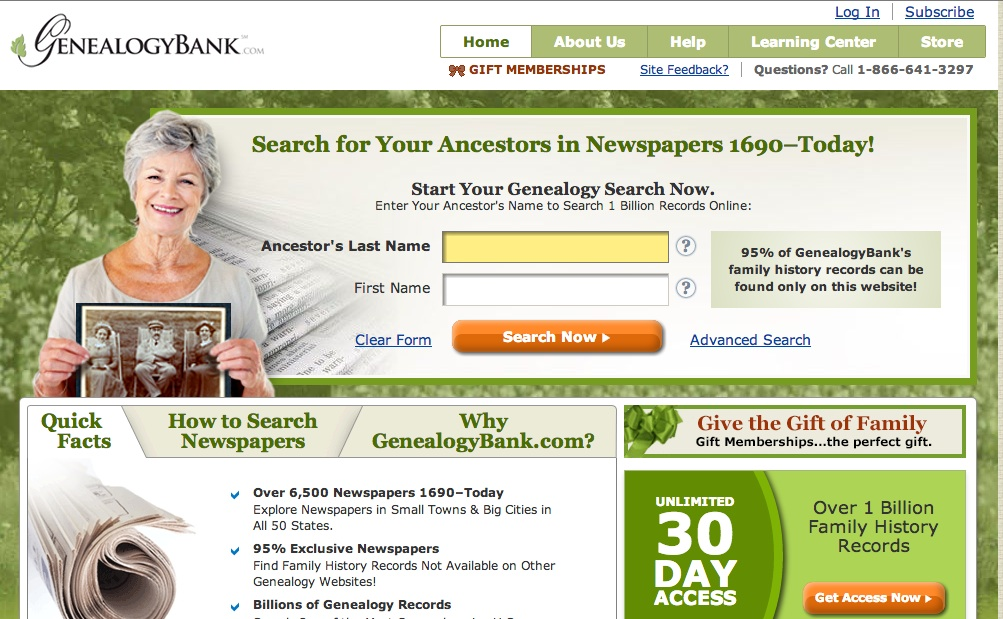
\includegraphics[scale=0.2]{genealogy.jpg}
\end{center}
\end{figure}
\item Finding influential people from historic newspaper archives- a novel problem
\end{itemize}
\end{frame}


%PROBLEM DESCRIPTION
\section{Problem Description}
\begin{frame}
\frametitle{Problem Description}
\textbf{Aim}: To find ``influential" people from historical news OCR archives where
an influential person can be defined as:\\


``A person whose actions and opinions strongly influence a course of events"\\  \vspace{0.5in}

\pause
Divided into subproblems:
\begin{itemize}
\pause
\item Spell Correction and Cleaning of OCR text
\pause
\item Development of a People Gazetteer-an organized structure to ease the process of identification of influential people
\pause
\item Influential People Identification-define the criteria to identify and rank people as ``influential".
\end{itemize}

\end{frame}


%NOVEL CONTRIBUTION
\section{Novel Contribution}
\begin{frame}
\frametitle{Novel Contribution}
\begin{itemize}
\item A novel Spell Correction Evaluation (SCE) algorithm for measuring performance of Spelling Correction
\item Development of People Gazetteer - an organized dictionary of people names and a list of news articles of their occurrence along with the corresponding topic label of each article which can be used to identify and rank influential people
\item Define an Influential Person Index (IPI) and metrics for its calculation to identify and rank influential people from the People Gazetteer
\end{itemize}
\end{frame}


%RELATED WORK
\section{Related Work}
\begin{frame}
\frametitle{Related Work}
\begin{itemize}
\item
GATE gazetteers\footnote{http://gate.ac.uk/sale/tao/splitch13.html} define gazetteers as set of lists containing names of entities such as cities, organizations, days of week, etc
\item
Gazetteers have been used as a processing resource to find occurrence of entity names in text\cite{carlson2009learning}\cite{zhang2009novel} (Example: Named Entity Recognition)
\item
Influential people identification has been done mostly in the field of social networking, marketing and diffusion research\cite{cha2010measuring}\cite{agarwal2008identifying}
\item
 Number of votes, tweets, comments, followers, etc are common parameters used for defining influence but not applicable to the newspaper environment 
\end{itemize} 

\end{frame}

 
%SOLUTION FRAMEWORK
\section{Solution Framework}
\begin{frame}

\frametitle{Solution Framework}
\begin{figure}[ht]
\begin{center}
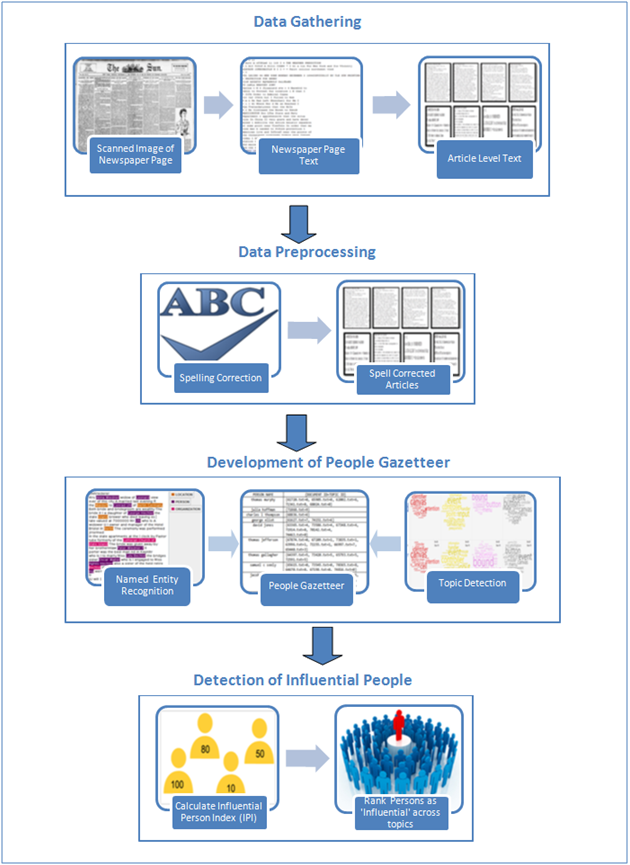
\includegraphics[scale=0.35]{images/framework3.png}
\end{center}
\end{figure}

\end{frame}

%DATA DESCRIPTION
\subsection{Data Gathering}
\tableofcontents[currentsection,currentsubsection]

\begin{frame}

\frametitle{Data Gathering}
\begin{itemize}
\item \textbf{Data Source} : Chronicling America - provides scanned OCR newspaper pages of American newspapers published between 1836 and 1922 
\item \textbf{Data Statistics} : 14020 news articles of ``The Sun" newspaper published between November-December 1894 consisting of 8 million tokens
\item \textbf{Data Characteristics} : News articles consist of one or more OCR errors of the types- Real word, Non-real word, Non-word, Word Split and Join and New line errors
\end{itemize}
\end{frame} 

%DATA PREPROCESSING
\subsection{Data Preprocessing}
\tableofcontents[currentsection,currentsubsection]

\begin{frame}
\frametitle{Data Preprocessing}
\begin{itemize}
\item
Required to deal with OCR errors in the news articles
\item
Edit distance algorithm used for spelling correction of non-real and non-word OCR errors using precompiled dictionary for look-up
\item
Person name correction is improved by enhancing dictionary with people names by running Stanford NER-CRF parser on subsets of the ClueWeb12 dataset available as a part of TREC 2013 Crowdsourcing track
\end{itemize}
\end{frame}

\begin{frame}
\frametitle{Spelling Correction Algorithm}

\begin{itemize}
\item ``Edit distance" corresponds to the minimum number of insertion, deletion and substitution required to transform one string into another\\
\begin{center}
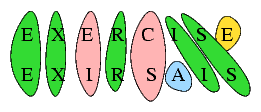
\includegraphics[scale=0.35]{images/edit2.png}
\end{center}
\item String Edit distance algorithm for spelling correction:
\begin{figure}[ht]
\begin{center}
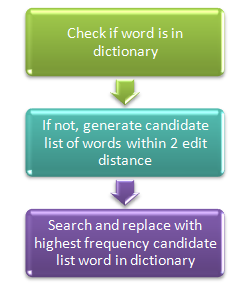
\includegraphics[scale=0.5]{images/editdistance.png}
\end{center}
\end{figure}
%\item Precompiled dictionary is used to search for candidate list of words within edit distance 2 from the word to be corrected
%\item Word correction is done by replacement with the highest frequency word and lowest edit distance among the candidate list of words

\end{itemize}
\end{frame}

\begin{frame}[allowframebreaks]
\frametitle{Spelling Correction Evaluation}

\begin{itemize}
\item
Required to measure the performance of spelling correction\\ \vspace{0.2in}
\item
Evaluation Parameters:
\end{itemize}
\begin{enumerate}
\item \alert{ Accuracy} : measures the percentage of actual errors that get corrected in the OCR text after spelling correction and defined as follows:
$$Accuracy=  \dfrac{TP+FP} {TP+ FP + TN + FN}$$


where, 

$TP$=Number of True Positives,

$TN$=Number of True Negatives,

 $FP$=Number of False Positives,

 $FN$=Number of False Negatives.



\item \alert{Time taken} to run Spelling Correction Algorithm
\item \alert{Person Names Detection Rate} (PNDR) : defined as the ratio of person names recognized through Named Entity Recognition (NER) before spelling correction process and the total number of person names recognized in the original newspaper articles
$$PNDR=\dfrac{ \text{Person Names recognized before/after spelling correction}} {\text{ Person Names recognized in original newspaper articles}} $$
\end{enumerate}
\end{frame}


\begin{frame}
\frametitle{Spelling Correction Evaluation (SCE) Algorithm}
\begin{itemize}
\item Word by word correspondence between corrected and original dataset not possible because of Word Split and Join errors in OCR dataset
\item SCE algorithm performs word by word automatic evaluation on post spell corrected OCR dataset using an n-word grams approach
%\item Algorithm uses an n-word grams approach by considering a window of k words before and after each word in the original text for each word in the corrected text
%\item Each word in the corrected text is marked as a True Positive, True Negative, False Positive, False Negative based on whether the spelling had been corrected and if a match is found in the k words window of the original text
\end{itemize}

\begin{columns}
\column{0.7\textwidth}
%\begin{figure} [!htb]
\centering
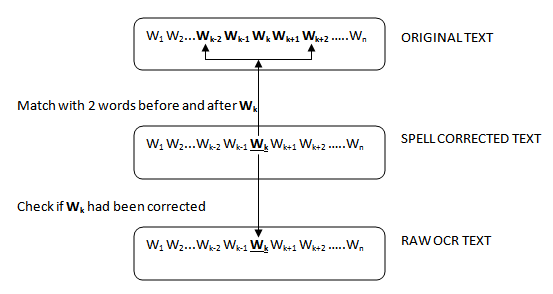
\includegraphics[scale=0.5]{images/ngram}
%\end{figure}

\column{0.3\textwidth}
%\begin{figure} 
\centering
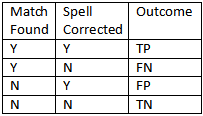
\includegraphics[scale=0.5]{images/ngram2}
%\caption{Schematic diagram for alignment of spell corrected article text with original article text for a word $W_{k}$}
%\end{figure}

\end{columns}
\begin{figure}
\caption{Schematic diagram for alignment of spell corrected article text with original article text for a word $W_{k}$}
\end{figure}
\end{frame}



\begin{frame}
\frametitle{Example}
\begin{block}{Line text from 3 versions of a news article:}
OcrLine= \textit{Irnniluttry iiownllllnu at tilchmond}\\

CorrectedLine= \textit{Irnniluttry iiownllllnu at Richmond}\\

OriginalLine= \textit{Grand jury now sitting at Richmond} 
\end{block}

\begin{table}[bt]
\begin{tabular}{|p{2.5cm}|p{4.5cm}|p{2cm}|} \hline
\textbf{Word in Corrected Line} & \textbf{Corresponding Word Window in Original Line}& \textbf{Result} \\ \hline
Irnniluttry & Grand jury now & FN \\ \hline
iiownllllnu & Grand jury now sitting & FN \\ \hline
at & Grand jury now sitting at & TN \\ \hline
Richmond  &  sitting at Richmond & TP \\ \hline
\end{tabular}
\end{table}
\end{frame}

\begin{frame}
\frametitle{Spelling Correction Evaluation Results}
\begin{itemize}
\item
SCE algorithm tested on 50 spell corrected articles using 3 versions of each article: Original text, Raw OCR text and Spell Corrected text

\begin{block}{}
Accuracy :  $72.7 \%$\\
Time taken : 9 seconds on average per article
\end{block}

\begin{block}{}
PNDR from Raw OCR : 72.5\% \\

PNDR from spell corrected text : 63.3\% \\

PNDR from spell corrected text with enhanced people names dictionary : 82.5\% \\
\end{block}
\item
Results indicate less accuracy due to large number of incorrected OCR errors and usefulness of person names dictionary for spell correction and person names detection 
\end{itemize}
\end{frame}

\begin{frame}
\frametitle{Discussion}
\begin{itemize}
\item
Spelling Correction accuracy can be improved by correcting other OCR errors like New Line and Word Split and Join errors
\item
 Choice of a dictionary for the edit distance algorithm affects the results of spelling correction and PNDR using enhanced person names dictionary
\item
SCE algorithm can be used to compare among multiple spell correction algorithms and decide which one suits the dataset better and gives best accuracy

\end{itemize}
\end{frame}


\subsection{Development of People Gazetteer}
\tableofcontents[currentsection,currentsubsection]
\begin{frame}
\frametitle{Development of People Gazetteer}
\begin{itemize}
\item
People Gazetteer: an organized structure developed to ease the process of influential people identification
\item
Two step process:
\begin{enumerate}
\item
Person Named Entity Recognition (PNER)-
 Extraction of person names from the news articles dataset using Named Entity Recognition
\item
Topic Detection-Assignment of topics to news articles using LDA model
\end{enumerate}
\end{itemize}
\end{frame}



\begin{frame}
\frametitle{PNER}
\begin{itemize}
\item
 Stanford CRF-NER used for the process of Named Entity Recognition 
\item
Only multi-term person entities are analyzed \\
Example: \alert {Henry} is ignored while \alert{Henry Smith} is stored
\item
Inverted Index is created to link person entities with the list of news articles in which they occur
\item
38426 person entities recognized from 14020 news articles 

\end{itemize}
\end{frame}


\begin{frame}
\frametitle{Person Categories}
 Extracted person entities are divided into following categories for separate analysis of each category:
\begin{table}[bt]
\begin{tabular}{|p{3.5cm}|p{3cm}|p{2cm}|} \hline
\textbf{Person Category} & \textbf{Number of news articles}& \textbf{Statistics from dataset} \\ \hline
Marginally Influential & less than 4 & 38066 \\ \hline
Medium Influential & 4 to 15 & 344 \\ \hline
Highly Influential & more than 15 & 16 \\ \hline
\end{tabular}
\end{table}
\end{frame}


\begin{frame}
\frametitle{Topic Detection}
\begin{itemize}
\item
\alert{Topic} : a set of words which describe what any document is about
\item
\alert{Topic Detection}: use topic modelling algorithm for examining a set of documents and discover main topics occurring across the documents as well as the balance of topics in each document based on the statistics of the words in the complete document set
\item
\alert{LDA} :  generative probabilistic model in which documents exhibit multiple topics and each topic is a distribution over a fixed vocabulary
\item
\alert{AD-LDA} : approximate distributed LDA model that uses distributed computation on multiple processors to infer document topics and is faster than the simple LDA approach
\end{itemize}
\end{frame}

\begin{frame}
\frametitle{Topic Model Evaluation}
\begin{itemize}
\item
Evaluation required to decide parameters to be used for topic modeling
\item
Evaluation measure:	\alert{Perplexity}\\
\begin{enumerate}
\item 
It indicates how surprised a trained model is when given a held out test data and calculated as follows:

$$Perplexity= \exp(-\dfrac{\text{Log Likelihood of held-out test set}}{\text{Number of tokens in held-out test set}})$$

\item
It is a decreasing function of the log likelihood of the unseen documents 
\item
Lower the perplexity, better is the topic model
\end{enumerate}
\end{itemize}
\end{frame}


\begin{frame}[allowframebreaks]
\frametitle{Topic Model Evaluation Results}
\begin{figure}[ht]
\begin{center}
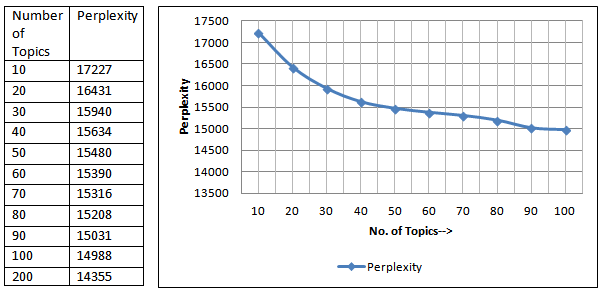
\includegraphics[scale=0.5]{images/topicperplex2}
\caption{Test Set Perplexity versus Number of Topics for a random $90-10$ split of the data using AD-LDA. The maximum number of words in each topic is $20$, number of iterations $500$ and the number of processors $4$ for this experiment.}
\end{center}
\end{figure}

\begin{itemize}
\item
 Variability in perplexity with respect to the number of topics was found to be much greater than the variability due to the number of processors or number of iterations

\item
Two models finalized from topic detection and used for developing people gazetteer:
\begin{enumerate}
 \item \textbf{30 Topics LDA Model} : Number of topics = 30, Number of iterations = 500, Number of threads=4
 \item \textbf{100 Topics LDA Model} : Number of topics = 100, Number of iterations = 500, Number of threads=4
\end{enumerate}
\end{itemize}
\end{frame}



\begin{frame}
\frametitle{Output of People Gazetteer}
\begin{itemize}
\item
Person Name + Document List + Document Topic =$>$ People Gazetteer
%\item The list of articles obtained for each person entity after application of PNER and highest scoring topic assigned to each article during Topic Detection are combined to obtain People Gazetteer
%\item Two people gazetteers are obtained for topic model settings of 30 Topics LDA Model and 100 Topics LDA Model respectively
\end{itemize}
\begin{figure}[ht]
\begin{center}
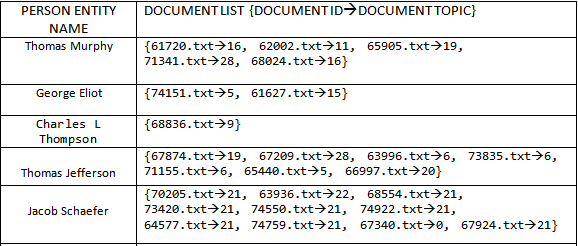
\includegraphics[scale=0.7]{images/gaz2.png}
\caption{Snapshot of the people gazetteer using 30 Topics LDA Model where each person entity is associated with a list consisting of a text Document ID and its corresponding Topic ID.}
\end{center}
\end{figure}
\end{frame}

\begin{frame}[allowframebreaks]
\frametitle{Discussion}
\begin{itemize}
\item
Lack of punctuation in the OCR dataset leads to high number of false positives as well as missing recognition of several person entities during PNER

\begin{block}{Example}
 ``They gave money to Ronn Collector A Augustus Healy Speaker has been appointed.." leading to the recognition of person entity ``Ronn Collector A Augustus Healy Speaker"
\end{block}	 
\item
Person Named Entity Disambiguation is required to differentiate among persons with similar names in news articles
% a hard problem to solve since persons with similar names can occur in multiple topic related articles in newspapers
\item

Co-reference Resolution of person names needs to be performed to link multiple ways in which a single person is addressed\\

\begin{block}{Example}
``William Schmittberger",``Captain William" recognized as separate person entities in an article
\end{block}
\item
The LDA topic detection model is also not geared to be used on OCR dataset directly since it recognizes some topics having completely meaningless words\\

\begin{block}{Example}
\begin{enumerate}
\item
 air ran ur fur ui full tt al tl late mr ant liar art lay told met ti tr\\
 \item
 la lu ot lo tu au tb ta ha tea day al aa ut ar uu wa tt te
\end{enumerate}
\end{block}
\end{itemize}
\end{frame}


\subsection{Identifying Influential People}
\tableofcontents[currentsection,currentsubsection]
\begin{frame}
\frametitle{Identification of Influential People}
\begin{itemize}
\item
Define Document Index (DI) to measure effect of each document on a person's influence score
\item
Calculate Influential Person Index (IPI) for each person entity based on the maximum DI in their document list
\item
Rank person entities in the people gazetteer in decreasing order of IPI
\end{itemize}
\end{frame}

\begin{frame}[allowframebreaks]
\frametitle{Document Index}
\begin{itemize}
\item
Measures how each document in the person entity's associated list of documents affects his influence score
\item
Parameters for estimating DI:
\begin{enumerate}
\item
\alert{ Normalized Document Length} (NDL) : normalized number of tokens contained in a news article

$$\text{ NDL}=\dfrac{\text{Document Length}} {\text{Maximum Document Length in the dataset}}$$

\item
\alert{Normalized Term Frequency} (NTF) : normalized number of occurrences of a person's name in a news article\\ \vspace{0.15in}

$\text{NTF}=	1	+\log	$(TF of person entity in current article)\\ \vspace{0.1in}

\item  
\alert{Number of similar articles} (NSIM) :  proportion of topic similar articles for a news article in a person's list

$$NSIM= \dfrac{\text{Number of topic similar articles}} {\text{Total number of articles in the person's document list}}$$

\end{enumerate}

\item
Formula for estimating DI:

\begin{block}{}
$$DI = w_a . NDL + w_b . NSIM + w_c . NTF $$
\end{block}
where, $w_a$,$ w_b$ and $w_c$ are the weights associated with each of the parameters NDL, NSIM and NTF respectively

\item
DI is a heuristic measure of these three parameters where each of the parameters can be weighted as per dataset characteristics and user requirements
\end{itemize}
\end{frame}

\begin{frame}
\frametitle{Influential Person Index}
\begin{itemize}
\item
An index calculated for each person entity in order to measure its influence in the news dataset and calculate its influential score
\item
Formula for calculation of IPI:
\begin{block}{}
$$IPI= max DI(d_1, d_2, ...,d_n)+ UniqT$$
\end{block}
where, \\
 $max DI(d_1, d_2, ...,d_n)$ = Maximum Document Index of a document $d_i$ in a person entity's list of  $n$ articles

$$UniqT = \dfrac{\text{Number of Unique Article Topics in a person entity's list}}{\text{Total Number of Topics in the corpus}}$$

\end{itemize}
\end{frame}

\section{Results}
\begin{frame}[allowframebreaks]
\frametitle{Comparison Across Influential Person Lists}
Two ranked influential person lists, namely $L_1$ and $L_2$ are obtained after calculation of IPI from each people gazetteer using 30 Topics and 100 Topics LDA Model respectively
\begin{figure}[h]
\begin{center}
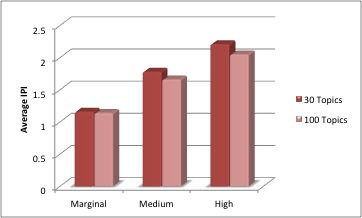
\includegraphics[scale=0.5]{IPIChart}
\end{center}
\caption{Comparison of the Average IPI for two ranked lists $L_1$ and $L_2$ using $30$ and $100$ topic LDA model respectively.}
\end{figure}


\begin{table}
\begin{center}
    \begin{tabular}{|p{2cm}|p{2cm}|p{2cm}|p{2cm}|}
    \hline
    \textbf{Person Category}   & \textbf{Average Number of Documents}   &  \textbf{Average Document Length}	&  \textbf{Average Term Frequency}	\\  \hline
Marginal  & 1.04 & 2119.6 & 1.07 	\\ \hline
Medium  & 5.75 & 1976.3 & 6.68  \\ \hline
High  & 22.8 & 2971.5 & 29.870	 \\	\hline 
  \end{tabular}
  \end{center}
    \caption {Average statistics for each Person Category of People Gazetteer across 2 Topic Models}
\end{table}
\begin{itemize}
\item
Results indicate the fact that highly influential category people are more susceptible to change in number of topics
\item
Number of articles of occurrence for a person entity cannot be used uniquely to determine a person as ``influential"
\end{itemize}
\end{frame}

\begin{frame}[allowframebreaks]
    \scalebox{0.55}{\begin{minipage}{1.8\textwidth}

\begin{table}
\begin{center}
\begin{tabular}{|p{2cm}|l|p{1.5cm}|p{1.5cm}|l|l|l|p{3cm}|l|l|}
\hline
Person Name    & IPI  & Number of Articles & Person Category & NDL  & NTF  & NSIM & TOPIC WORDS                                                          & UniqT & Rank \\ \hline
capt creeten   & 3.38 & 10                 & Medium          & 0.56 & 1.95 & 0.8  & mr court police judge justice case yesterday street district         & 0.06  & 1    \\ \hline
capt hankey    & 3.02 & 6                  & Medium          & 0.68 & 1.6  & 0.66 & club game team play football half ball left college back             & 0.06  & 2    \\ \hline
capt pinckney  & 2.93 & 3                  & Marginal        & 0.38 & 1.84 & 0.67 & man ho men night back wa room left house told bad                    & 0.03  & 3    \\ \hline
\end{tabular}
\end{center}
\end{table}



\begin{table}[!h]
\begin{center}
\begin{tabular}{|p{2cm}|l|p{1.5cm}|p{1.5cm}|l|l|l|p{3cm}|l|l|}
\hline
Person Name    & IPI  & Number of Articles & Person Category        & NDL  & NTF  & NSIM & Topic Words                                                                 & UniqT & Rank \\ \hline
capt creeten   & 3.33 & 10                 & Medium     & 0.56 & 1.95 & 0.8  & mr police witness committee capt asked captain money inspector paid         & 0.02  & 1    \\ \hline
mrs martin     & 3.23 & 8                  & Medium     & 0.20 & 2.38 & 0.5  & mrs mr years wife home house ago woman city died                            & 0.02  & 2    \\ \hline
alexander iii  & 3.09 & 31                 & High     & 0.49 & 2.04 & 0.48 & emperor prince french alexander czar london nov government imperial russian & 0.07  & 3    \\ \hline
\end{tabular}
\end{center}
\caption{Comparison of top 3 influential persons for two ranked lists $L_1$ and $L_2$ using $30$ and $100$ topic LDA model respectively.}
\end{table}

\end{minipage}}
\end{frame}

\begin{frame}
\frametitle{Evaluation}
\begin{itemize}
\item
No gold standard data available regarding influential persons  in the newspaper archives from November-December 1894
\item
Evaluation done through Wikipedia search of top 30 influential persons of ranked lists L1 and L2
\end{itemize}

\begin{block}{Evaluation Results}
 16 and 14 out of the top 30 person entities were found to be influential and popular in the 19th century across topic categories like theatre, sports, government, shipping, etc. in lists L1 and L2 respectively
\end{block}
\end{frame}



\begin{frame}
\frametitle{Influential Persons}
\begin{figure}
\centering
 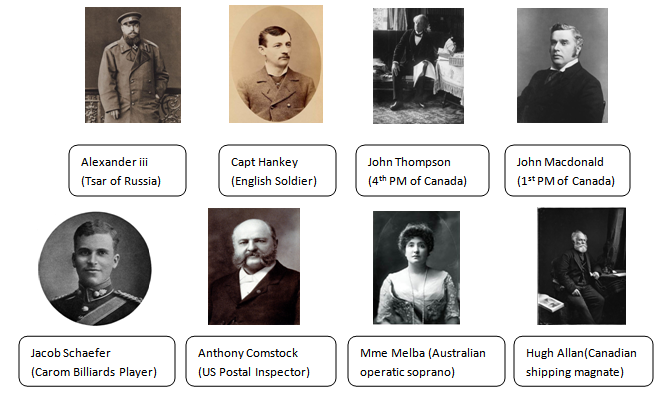
\includegraphics[scale=0.6]{images/ip}
\caption{Some of the top 30 influential persons found during evaluation from Wikipedia}

\end{figure}
\end{frame}



\begin{frame}
\frametitle{Discussion}
\begin{itemize}
\item
 Linear combination of  parameters used in calculation of DI and IPI
% assigned equal values to the weights associated with each of them by not favoring any specific parameter

\item
Parameters for calculation of DI and IPI can also be learned by performing regression analysis
% manually developed sample of topmost influential people and obtaining the complete list of ranked influential people based on the learned parameters.

\item
Effect of different ways of normalizing parameters on ranking of influential people needs to be analyzed

\item
The topmost influential people contain several false positives due to OCR errors and PNER issues\\
\alert{Example} : ``van cortlandt", ``ann arbor" , ``sandy hook",``mrs martins" , ``mrs oakes"

\end{itemize}
\end{frame}

\section{Conclusion and Future Work}
\begin{frame}
\frametitle{Conclusion and Future Work}
\begin{itemize}
\item
Proposed a novel approach and highlighted challenges for finding influential people from historical OCR news repository

\item
Non-heuristic estimation for finding influential persons possible through optimization approaches such as unsupervised multiple instance clustering\cite{zhang2009m3ic}
\pause
\item
 Algorithm is a combination of Constrained Concave-Convex Procedure and Cutting Plane method with faster convergence
\pause
\item 
Cluster person entities into ``influential" or ``non-influential" by considering each person entity as a bag with articles of their occurrence as the instances for each bag

\end{itemize}
\end{frame}

\begin{frame}

\begin{center}
\usebeamerfont*{frametitle} \usebeamercolor[fg]{frametitle}
\Huge Thank You!\\ \vspace{0.2in}
Questions??
\end{center}

\end{frame}

\section*{References}
\begin{frame}

\frametitle{References}

\scriptsize{\bibliographystyle{acm}}

\bibliography{aayushee2} %bibtex file name without .bib extension

\end{frame}


%EXTRA SLIDES


\begin{frame}
    \scalebox{0.65}{\begin{minipage}{1.53846\textwidth}

\begin{algorithm}[H]
\caption{MatchWordGrams function of SCE Algorithm for measuring accuracy }
\begin{algorithmic}
\Function {MatchWordGrams}{OcrLine, CorrectedLine, OriginalLine, jstart, jend, i}
  
 \For{(int j=jstart; j$<$jend; j++)}
  {
    \If{ ((CorrectedLine[i].equals(OriginalLine[j]))\&\&(!(OcrLine[i].equals(CorrectedLine[i]))))}
     {
	  $tp=tp+1$\;
	  flag0=false\;
	 \Return $tp$\;
	  }
	\ElseIf{((CorrectedLine[i].equals(OriginalLine[j]))\&\&(OcrLine[i].equals(CorrectedLine[i])))}
	      {
		 $tn=tn+1$\;
		  flag1=false\;
		\Return $tn$\;
	      }
}

	 \If{(!(OcrLine[i].equals(CorrectedLine[i]))\&\&flag0==true)}
	 {
		    $fp=fp+1$\;
		   \Return $fp$\;
            }
	 
	 \ElseIf{((OcrLine[i].equals(CorrectedLine[i])) \&\& flag1==true)}
	 {
		    $fn=fn+1$\;
		   \Return $fn$\;
	 }
\EndFunction
\end{algorithmic}
\end{algorithm}%
\end{minipage}}
\end{frame}

\begin{frame}
   \scalebox{0.65}{\begin{minipage}{1.53846\textwidth}

\begin{table}
 
   \begin{tabular}{|p{1cm}|p{16cm}|}

    \hline
    TOPIC ID & TOPIC WORDS                                                                                                                                           \\ \hline
    1        & total ii won club score night ran furlough alleys tournament time   mile fourth rolled curling scores race national game                              \\ \hline
    2        & la lu ot lo tu au tb ta ha tea day al aa ut ar uu wa tt te                                                                                            \\ \hline
    3        & iii lie tin nail tn lit hut ill ii nn thu tu anti thin inn hit lu lo   nut                                                                            \\ \hline
    4        & line street feet point western easterly northerly feel southerly   distance place distant lo fret hue beginning laid early felt                       \\ \hline
    5        & opera theatre music company week play stage evening night performance   concert mme audience manager season de orchestra house miss                   \\ \hline
    6        & great people life man women good country world american part ot ha   made la years make long place bad                                                \\ \hline
    7        & election mr party republican state district vote democratic county senator   elected city committee mayor political candidate majority york democrats \\ \hline
    8        & time ho work tn men city bo lie anti day thin long thu made part ago   lot york make                                                                  \\ \hline
    9        & st room av sun wife board front lo december rent lot november sunday   ht west ar house private si                                                    \\ \hline
    10       & dr book st story books cloth author cure free work york blood   illustrated remedy goods medical library health price                                 \\ \hline
    11       & church dr father funeral school st college sunday year rev catholic pastor services late service held society holy clock                              \\ \hline
    12       & horse race class horses won racing years prize record year show ring track mile money jockey trotting trotter ran                                     \\ \hline
    13       & cent year week pf market total net stock today central st ft lit sales short cotton ohio lot month                                                    \\ \hline
    14       & white water indian black long found thu big dog time ground wild tree killed birds bird day great lake                                                \\ \hline
    15       & price black silk goods prices ladies worth dress fine white full tea quality style wool made fancy cloth fur                                          \\ \hline
     \end{tabular}
\caption{ Topic ID and words obtained from the 30 Topics LDA model.}
\end{table}
\end{minipage}}
\end{frame}

\begin{frame}

   \scalebox{0.65}{\begin{minipage}{1.53846\textwidth}

\begin{table}
 
   \begin{tabular}{|p{1cm}|p{16cm}|}

    \hline
    TOPIC ID & TOPIC WORDS                                                                                                                                           \\ \hline
   16       & street mrs mr avenue wife house miss yesterday years home woman night ago husband found died daughter children mother                                 \\ \hline
    17       & war american government army chinese japanese china japan foreign united nov emperor states prince minister military french port navy                 \\ \hline
    18       & feet north minutes avenue boundary seconds degrees west york minute degree point east south feel city angle county laid                               \\ \hline
    19       & man ho men night back wa room left house told bad door found turned place ran lie front morning                                                       \\ \hline
    20       & water feet building boat company car train road fire miles railroad island work line city great river built bridge                                    \\ \hline
    21       & club game team play football half ball left college back yale played harvard line eleven men match yacht field                                        \\ \hline
    22       & ii iii ill lit ll si ti il im vi st iv ft mi li till lull lui oil                                                                                     \\ \hline
    23       & bank money national gold amount notes banks hank business treasury account cent paid bonds note currency company stock estate                         \\ \hline
    24       & mr john william york henry charles james club city ii george dec dr thomas smith jr brooklyn van held                                                 \\ \hline
    25       & piano st rooms car york daily chicago city sunday upright parlor furnished broadway hotel av west train brooklyn monthly                              \\ \hline
    26       & york daily steamship nov directed letter dec fur orleans al steamer walls letters close australia china japan city london                             \\ \hline
    27       & mr court police judge justice case yesterday street district witness jury charge asked attorney trial arrested lawyer told office                     \\ \hline
    28       & mr law present made public year state committee president secretary bill report states con tin united number meeting york                             \\ \hline
    29       & air ran ur fur ui full tt al tl late mr ant liar art lay told met ti tr                                                                               \\ \hline
    30       & company york trust bonds city cent railroad mortgage interest wall bond stock street st central january coupon committee jan                          \\ \hline
    \end{tabular}
\caption{ Topic ID and words obtained from the 30 Topics LDA model.}
\end{table}
\end{minipage}}
\end{frame}






\end{document}